\chapter{仮説}
\label{proposed}
%どうやったら解けると考えているか (検証可能なように書く)

本章では仮説について述べる。

\section{概要}
本研究では、利用規約の読解支援のために、以前同意した利用規約を記録し、それに類似する条文を読んだときに類似していることを検出し、それ以外に注目することで、利用規約の読解時間の短縮ができるのではないかと考えた。

\subsection{利用規約類似文検出}
仮説のうち、類似条文を検出する部分について述べる。

図\ref{img:demo}では、イメージを示している。ここでは、提案するシステムを利用し始めて、初めに、A社の利用規約を読んだときは条文の背景が全て黄色で目立ち、次にB社の利用規約を読むと3がA社の1と類似する条文であるため、それ以外の条文が背景が黄色で目立ち、最後にC社の利用規約を読むと1,3,4,5が類似する条文であるため、2が背景が黄色で目立つイメージとなっている。
\label{sub:利用規約類似文検出}
\begin{figure}[h]
  \begin{center}
      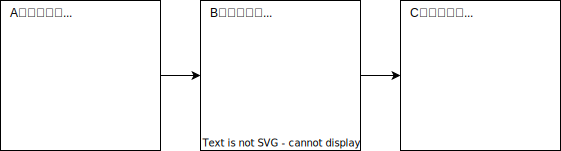
\includegraphics[width=15cm]{img/demo.drawio.png}
      \caption{類似条文検出のイメージ}
      \label{img:demo}
  \end{center}
\end{figure}

\subsection{利用規約警告検出}
\label{sub:利用規約警告検出}

%%% Local Variables:
%%% mode: japanese-latex
%%% TeX-master: "../bthesis"
%%% End:
